\section{ Electroweak Diboson Physics }	
\label{sec:EWKPheno}

In LHC, two types of physics processes, the QCD production at the order $\alpha_{S}^{2} \alpha_{EWK}^{4}$ and the EWK production at order $\alpha_{EWK}^6$ contribute to the production of di-$Z$ bosons in an association of two jets ($ZZjj$) \cite{CMSRun2ZZjj}. Figure \ref{fig:ZZjjFeynmanDiag_QCD} shows the Feynman diagram at leading order for the QCD ZZjj process, whereas figure \ref{fig:ZZjjFeynmanDiag_EWk} shows the Feynman diagram at leading order for the EWK production of ZZjj \cite{PowhegV2ZZjj}. The EWK production consists of two sets of interactions, first, the Vector Boson Scattering processes involving either triple (figure \ref{fig:ZZjjFeynmanDiag_EWk_a}) or quartic (figure \ref{fig:ZZjjFeynmanDiag_EWk_b}) self-interactions of the gauge-bosons, and second the diagrams featuring the Higgs bosons (figure \ref{fig:ZZjjFeynmanDiag_EWk_c} $\&$ \ref{fig:ZZjjFeynmanDiag_EWk_d}). The scattering amplitudes of the VBS processes involving longitudinally polarized vector bosons, grow quadratically with the center of mass energy ($\sqrt{s}$), eventually violating the unitarity bounds. The precise SM interference between the Higgs-featured process and the VBS process restores the unitarity  \cite{VBSWWWW}. As discussed in Section \ref{subsubsec:HiggsMech}, the massive $W$ and $Z$ bosons get their masses via the BEH mechanism through EWSB. As a consequence of EWSB, the $W$ and $Z$ bosons acquire an additional degree of freedom (the longitudinal polarization mode) whose scattering interfere with the Higgs featured processes. Thus, the study of electroweak production of the di-$Z$ bosons in association with two jets provides a direct probe of the EWSB, which is at the heart of the SM \cite{CMSRun2ZZjj}. 

\begin{figure}[!htbp]
  \begin{center}
  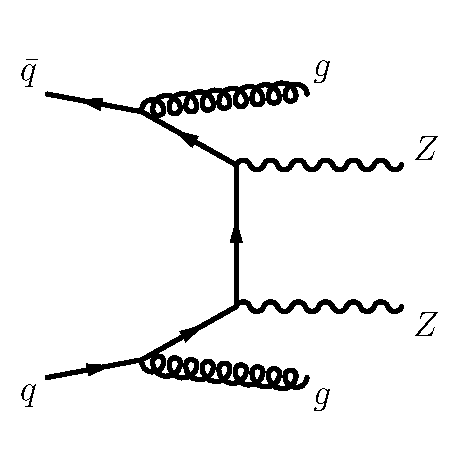
\includegraphics[width=0.31\textwidth]{figures/Theory/diagramQCDZZjjqq.pdf}
  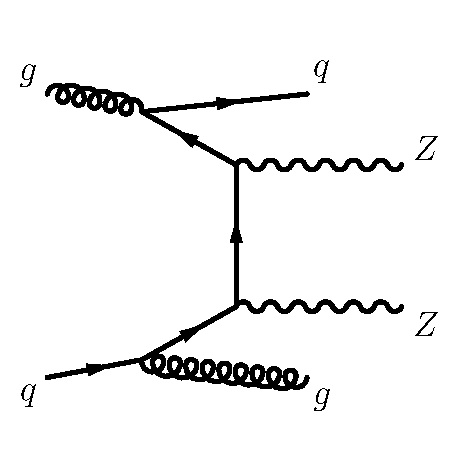
\includegraphics[width=0.31\textwidth]{figures/Theory/diagramQCDZZjjqg.pdf}
  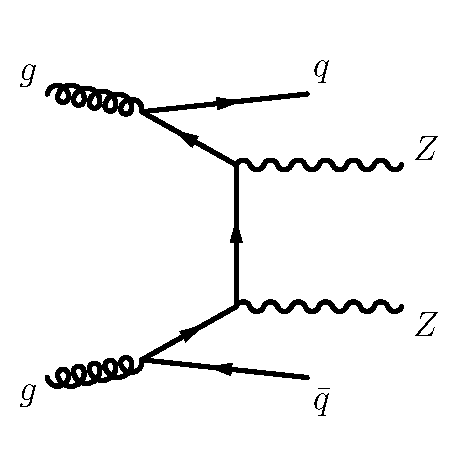
\includegraphics[width=0.31\textwidth]{figures/Theory/diagramQCDZZjjgg.pdf}\\
  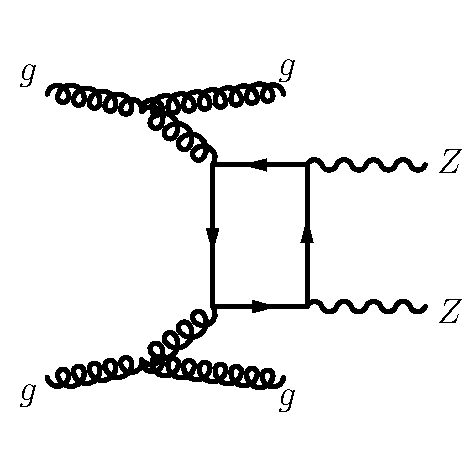
\includegraphics[width=0.31\textwidth]{figures/Theory/diagramQCDZZjjbox.pdf}
  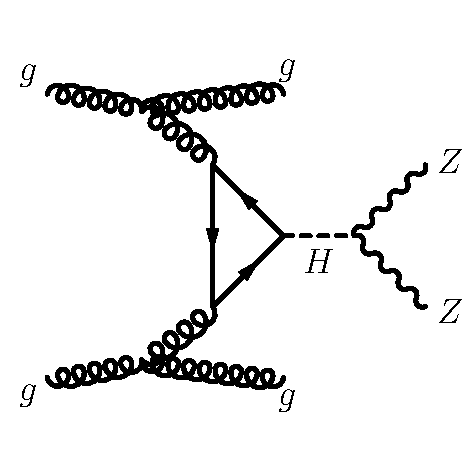
\includegraphics[width=0.31\textwidth]{figures/Theory/diagramQCDZZjjggH.pdf}\\
  \end{center}
  \caption{Typical diagrams for the QCD $\alpha_{S}^2\alpha_{EWK}^{4}$ production of $ZZjj$. \label{fig:ZZjjFeynmanDiag_QCD}}
 \end{figure}
 
\begin{figure}[ht]
\begin{subfigure}{.48\textwidth}
  \centering
  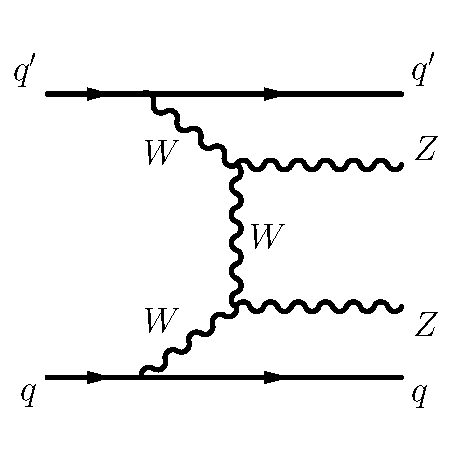
\includegraphics[width=.8\linewidth]{figures/Theory/diagramEWZZjjTGC.pdf}  
  \caption{ZZjj production with two triple gauge coupling (TGC) vertices.}
  \label{fig:ZZjjFeynmanDiag_EWk_a}
\end{subfigure}
\begin{subfigure}{.48\textwidth}
  \centering
  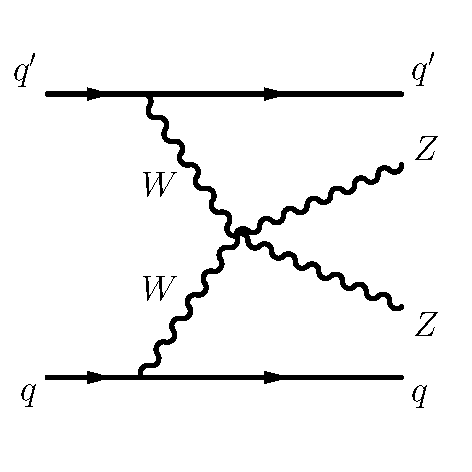
\includegraphics[width=.8\linewidth]{figures/Theory/diagramEWZZjjQGC.pdf}  \\
  \caption{ZZjj production with a quartic gauge coupling (QGC) vertex.}
  \label{fig:ZZjjFeynmanDiag_EWk_b}
\end{subfigure}
\begin{subfigure}{.48\textwidth}
  \centering
  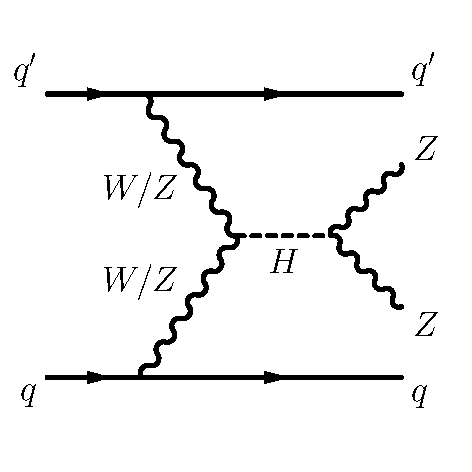
\includegraphics[width=.8\linewidth]{figures/Theory/diagramEWZZjjSchnHiggs.pdf}  
  \caption{s-channel Higgs ZZjj Production.}
  \label{fig:ZZjjFeynmanDiag_EWk_c}
\end{subfigure}
\begin{subfigure}{.48\textwidth}
  \centering
  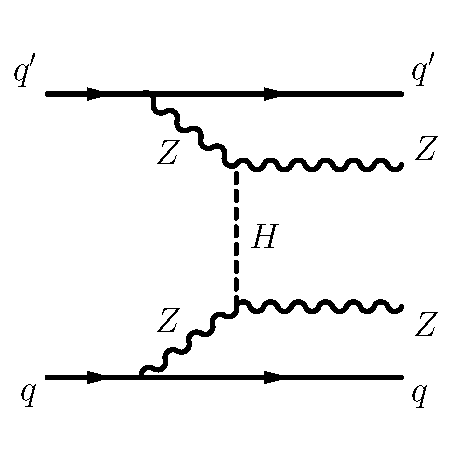
\includegraphics[width=.8\linewidth]{figures/Theory/diagramEWZZjjTchnHiggs.pdf}  
  \caption{t-channel Higgs ZZjj Production.}
  \label{fig:ZZjjFeynmanDiag_EWk_d}
\end{subfigure}\\
\caption{Feynman diagrams at LO for the EWK $\alpha_{EWK}^6$ production of $ZZjj$.}
\label{fig:ZZjjFeynmanDiag_EWk}
\end{figure}

The triple and quartic self-interactions of the gauge bosons arise from the non-Abelian structure of $SU(2)$ in the kinetic term $ \frac{1}{4} W^{a}_{\mu\nu} W^{\mu\nu}_{a}$ of the EWK Lagrangian in equation \ref{eqn:EWKLagrangian1}. Implementing the values of the field strength tensor $W^{a}_{\mu\nu}$ from equation \ref{eqn:SU2FST}, the relations of $W_{\mu}^{\pm}$ fields in equation \ref{eqn:RealWBosons}, and the relations of neutral gauge fields in equation \ref{eqn:NeutralGaugeBosons}, the triple and quartic self interaction terms become, 

\begin{equation}
\mathcal{L}_{3} = ie_{V=\gamma,Z} [ W^{+}_{\mu\nu} W^{-\mu} V^{\nu} - W^{-}_{\mu\nu} W^{+\mu} V^{\nu} + W_{\mu}^{+}W_{\nu}^{-}V^{\mu\nu} ] 
\label{eqn:L_TGC}
\end{equation}

\begin{equation}
\begin{array}{l}
\mathcal{L}_{4} = e^{2}_{W} [ W^{-}_{\mu}W^{+\mu}W^{-}_{\nu}W^{+\nu} - W^{-}_{\mu}W^{-\mu}W^{+}_{\nu}W^{+\nu} ] \\
 \hspace{10pt} + e^2_{V=\gamma,Z} [ W^{-}_{\mu}W^{+\mu}V_{\nu}V^{\nu} - W^{-}_{\mu}V^{\mu}W^{+}_{\nu}Z^{\nu} ] \\
  \hspace{10pt} + e_{\gamma}e_{Z} [ 2W^{-}_{\mu} W^{+\mu} Z_{\nu}A^{\nu} - W_{\mu}^{-}Z^{\mu}W^{+}_{\nu}A^{\nu} - W_{\mu}^{-}A^{\mu}W^{+}_{\nu}Z^{\nu} ]
\end{array}
\label{eqn:L_QGC}
\end{equation}

where, $e_{\gamma} = gsin\theta_{W}$; $e_{W} = \frac{e_{\gamma}}{2\sqrt{2}sin\theta_{W}}$ $\&$ $e_{Z} = e_{\gamma}cot\theta_{W}$ are the precise coupling strengths for vector boson self-interaction. Both triple and quartic neutral couplings such as $ZZZ$ or $ZZZZ$ are absent in the SM. 

Similarly, the couplings of Higgs to vector bosons are also predicted precisely by the BEH mechanism in equation \ref{eqn:LagBEHKin} as:

\begin{equation}
\mathcal{L}_{HVV} = \frac{m_{W}^2}{v^2} W^{+}_{\mu}W^{-\mu}h^{2} + \frac{m_{Z}^{2}}{v^2} Z_{\mu}Z^{\mu}h^{2}
\label{eqn:HVVCoupling}
\end{equation}

The EWK production of $ZZjj$ is extremely sensitive to any possible anomalous triple gauge couplings (aTGC), anomalous quartic gauge couplings (aQGC), or anomalous Higgs to vector boson coupling \cite{SensitivityNP} \cite{EboliModelaQGC} \cite{BSM_Simple2HDM} . Therefore, it is imperative to probe the high energy behavior of the EWK production of $ZZjj$ to seek possible deviations arising from the physics processes beyond the Standard Model (BSM). 

The EWK $ZZjj$ production with each $Z$ boson decaying to a pair of same-flavor opposite-sign (SFOS) lepton pairs is an extremely rare process. Moreover, with limited statistics in Run$-2$ the QCD background processes dominate the $ZZjj \rightarrow 4\ell jj$ final state \cite{ATLASZZjj}. Therefore, the differential cross-sections discussed in this thesis are measured in a VBS-enhanced phase space with a high fraction of events resulting from the EWK $ZZjj$ process. The enhanced phase space relies on the characteristic feature of the EWK process with two jets (jj) in the forward-backward region originating from the scattered quarks. These jets have large rapidity separation with no additional hadronic activity from the hard scattering between the two jets \cite{RapidityGapCite}. The decay of the two Z bosons into SFOS muons or electron pairs defines the final signature of the VBS-$ZZjj$-like event.
